% 76-28(76쪽) — $y=\sin\frac{1}{2}x\ (-\pi\le x\le 3\pi)$ 의 그래프와 두 직선 $y=\frac{3}{4}$, $y=-\frac{3}{4}$ · 네 교점 A, B, C, D 와 $x$좌표 $\alpha$, $\beta$, $\gamma$, $\delta$. 스캔 화질이 낮아 TikZ 로 다시 그림(원문 라벨·점선만).
\begin{tikzpicture}[line width=0.6pt, x=0.19cm, y=1.0cm]
  \draw[line width=0.5pt] (-5.3,0.75) -- (10.8,0.75);
  \draw[line width=0.5pt] (-5.3,-0.75) -- (10.8,-0.75);
  \draw[->, >=stealth, line width=0.7pt] (-5.3,0) -- (16.5,0) node[below=1pt] {$x$};
  \draw[->, >=stealth, line width=0.7pt] (0,-1.33) -- (0,1.72) node[left=1pt] {$y$};
  \draw[domain=-3.1416:9.4248, samples=170, smooth] plot (\x, {sin(28.6479*\x)});
  \draw[dotted, line width=0.5pt] (-3.1416,0) -- (-3.1416,-1);
  \draw[dotted, line width=0.5pt] (-1.696,0) -- (-1.696,-0.75);
  \draw[dotted, line width=0.5pt] (1.696,0) -- (1.696,0.75);
  \draw[dotted, line width=0.5pt] (4.587,0) -- (4.587,0.75);
  \draw[dotted, line width=0.5pt] (7.979,0) -- (7.979,-0.75);
  \draw[dotted, line width=0.5pt] (9.4248,0) -- (9.4248,-1);
  \fill (-3.1416,-1) circle (1.8pt);
  \fill (9.4248,-1) circle (1.8pt);
  \node[anchor=south east, font=\small] at (-3.05,0.05) {$-\pi$};
  \node[anchor=south east, font=\small] at (-0.4,0.05) {$\pt{O}$};
  \node[anchor=north, font=\small] at (-1.696,-0.03) {$\alpha$};
  \node[anchor=north, font=\small] at (1.696,-0.03) {$\beta$};
  \node[anchor=north, font=\small] at (4.587,-0.03) {$\gamma$};
  \node[anchor=south, font=\small] at (7.979,0.05) {$\delta$};
  \node[anchor=south west, font=\small] at (9.0,0.05) {$3\pi$};
  \node[anchor=north west, font=\small] at (-1.5,-0.78) {$\pt{A}$};
  \node[anchor=south east, font=\small] at (1.6,0.78) {$\pt{B}$};
  \node[anchor=south west, font=\small] at (4.75,0.78) {$\pt{C}$};
  \node[anchor=north east, font=\small] at (7.8,-0.78) {$\pt{D}$};
  \node[anchor=west, font=\small] at (11.0,0.75) {$y=\dfrac{3}{4}$};
  \node[anchor=west, font=\small] at (11.0,-0.75) {$y=-\dfrac{3}{4}$};
  \node[anchor=south west, font=\small] at (0.9,1.1) {$y=\sin\dfrac{1}{2}x$};
\end{tikzpicture}
